% Options for packages loaded elsewhere
\PassOptionsToPackage{unicode}{hyperref}
\PassOptionsToPackage{hyphens}{url}
%
\documentclass[
  10pt,
  ignorenonframetext,
]{beamer}
\usepackage{pgfpages}
\setbeamertemplate{caption}[numbered]
\setbeamertemplate{caption label separator}{: }
\setbeamercolor{caption name}{fg=normal text.fg}
\beamertemplatenavigationsymbolsempty
% Prevent slide breaks in the middle of a paragraph
\widowpenalties 1 10000
\raggedbottom
\setbeamertemplate{part page}{
  \centering
  \begin{beamercolorbox}[sep=16pt,center]{part title}
    \usebeamerfont{part title}\insertpart\par
  \end{beamercolorbox}
}
\setbeamertemplate{section page}{
  \centering
  \begin{beamercolorbox}[sep=12pt,center]{part title}
    \usebeamerfont{section title}\insertsection\par
  \end{beamercolorbox}
}
\setbeamertemplate{subsection page}{
  \centering
  \begin{beamercolorbox}[sep=8pt,center]{part title}
    \usebeamerfont{subsection title}\insertsubsection\par
  \end{beamercolorbox}
}
\AtBeginPart{
  \frame{\partpage}
}
\AtBeginSection{
  \ifbibliography
  \else
    \frame{\sectionpage}
  \fi
}
\AtBeginSubsection{
  \frame{\subsectionpage}
}
\usepackage{lmodern}
\usepackage{amssymb,amsmath}
\usepackage{ifxetex,ifluatex}
\ifnum 0\ifxetex 1\fi\ifluatex 1\fi=0 % if pdftex
  \usepackage[T1]{fontenc}
  \usepackage[utf8]{inputenc}
  \usepackage{textcomp} % provide euro and other symbols
\else % if luatex or xetex
  \usepackage{unicode-math}
  \defaultfontfeatures{Scale=MatchLowercase}
  \defaultfontfeatures[\rmfamily]{Ligatures=TeX,Scale=1}
\fi
\usetheme[]{metropolis}
% Use upquote if available, for straight quotes in verbatim environments
\IfFileExists{upquote.sty}{\usepackage{upquote}}{}
\IfFileExists{microtype.sty}{% use microtype if available
  \usepackage[]{microtype}
  \UseMicrotypeSet[protrusion]{basicmath} % disable protrusion for tt fonts
}{}
\makeatletter
\@ifundefined{KOMAClassName}{% if non-KOMA class
  \IfFileExists{parskip.sty}{%
    \usepackage{parskip}
  }{% else
    \setlength{\parindent}{0pt}
    \setlength{\parskip}{6pt plus 2pt minus 1pt}}
}{% if KOMA class
  \KOMAoptions{parskip=half}}
\makeatother
\usepackage{xcolor}
\IfFileExists{xurl.sty}{\usepackage{xurl}}{} % add URL line breaks if available
\IfFileExists{bookmark.sty}{\usepackage{bookmark}}{\usepackage{hyperref}}
\hypersetup{
  pdftitle={Course overview},
  hidelinks,
  pdfcreator={LaTeX via pandoc}}
\urlstyle{same} % disable monospaced font for URLs
\newif\ifbibliography
\usepackage{longtable,booktabs}
\usepackage{caption}
% Make caption package work with longtable
\makeatletter
\def\fnum@table{\tablename~\thetable}
\makeatother
\setlength{\emergencystretch}{3em} % prevent overfull lines
\providecommand{\tightlist}{%
  \setlength{\itemsep}{0pt}\setlength{\parskip}{0pt}}
\setcounter{secnumdepth}{-\maxdimen} % remove section numbering
\usepackage{hyperref}
\definecolor{links}{HTML}{2A1B81}
\hypersetup{colorlinks,linkcolor=,urlcolor=links}

\title{Course overview}
\author{}
\date{\vspace{-2.5em}}

\begin{document}
\frame{\titlepage}

\begin{frame}{Online coursebook}
\protect\hypertarget{online-coursebook}{}

\large

\begin{center}
\href{https://geanders.github.io/RProgrammingForResearch/}{https://geanders.github.io/RProgrammingForResearch/}
\end{center}

\end{frame}

\begin{frame}{Online coursebook}
\protect\hypertarget{online-coursebook-1}{}

\begin{center}\includegraphics[width=300pt]{../figures/get_slides} \end{center}

\end{frame}

\begin{frame}{ERHS 535 vs.~ERHS 581A3 / A4}
\protect\hypertarget{erhs-535-vs.-erhs-581a3-a4}{}

\begin{center}\includegraphics[width=300pt]{../figures/three_courses} \end{center}

\end{frame}

\begin{frame}{Time, place, and secondary instructor}
\protect\hypertarget{time-place-and-secondary-instructor}{}

\begin{itemize}
\tightlist
\item
  Time: Mondays and Wednesdays, \textbf{either} 10:00 am--11:00 am
  \textbf{or} 11:00 am--12:00 pm
\item
  Exceptions:

  \begin{itemize}
  \tightlist
  \item
    There will be no meeting on Labor Day (Monday, Sept.~7).
  \item
    There are no course meetings the week of Thanksgiving (week of
    Nov.~23).
  \end{itemize}
\item
  Place: Online through Zoom, YouTube, and
  \href{https://geanders.github.io/RProgrammingForResearch/}{online
  coursebook}
\end{itemize}

\end{frame}

\begin{frame}{Office hours}
\protect\hypertarget{office-hours}{}

\begin{itemize}
\tightlist
\item
  Office hours: Fridays, 10:00 am--11:00 am, online through Zoom
  (starting Friday, Sept.~4)
\item
  If needed, I will arrange a second time for weekly office hours to
  accommodate those who have a course or other formal obligation
  (regular lab meeting, regular experimental schedule) during the Friday
  morning office hours.
\end{itemize}

\end{frame}

\begin{frame}{Course book}
\protect\hypertarget{course-book}{}

\begin{itemize}
\tightlist
\item
  There is an online book for this course available at:
  \url{https://geanders.github.io/RProgrammingForResearch/}
\item
  This book includes course information, course notes, links to download
  PDFs of lecture slides, in-course exercises, homework assignments, and
  vocabulary lists for quizzes.
\item
  This online book is still in development, so it will be evolving
  throughout the semester. 
\end{itemize}

\end{frame}

\begin{frame}{Computer}
\protect\hypertarget{computer}{}

\begin{itemize}
\tightlist
\item
  You will need access to a computer and a reliable internet connection
  for this course.
\item
  If you do not have access to one of these, email me and we can try to
  figure something out.
\item
  If you are taking 535 or planning to continue to 581A4, we will be
  working with some large datasets. Please talk to me before the fifth
  week of class if you have limited space on your computer.
\end{itemize}

\end{frame}

\begin{frame}{Content}
\protect\hypertarget{content}{}

We will cover four large themes in this course:

\begin{itemize}
\tightlist
\item
  Entering and cleaning data
\item
  Exploring data
\item
  Reporting data results
\item
  Reproducible research
\end{itemize}

\end{frame}

\begin{frame}{Content}
\protect\hypertarget{content-1}{}

The first week covers preliminaries, and after that there will be
``cycles'' of covering these topics:

\begin{itemize}
\tightlist
\item
  \textbf{Preliminaries} Week 1
\item
  \textbf{Basic} Weeks 2--5 (ERHS 581A3 ends here)
\item
  \textbf{Intermediate} Weeks 6--9
\item
  \textbf{Advanced} Weeks 10--15
\item
  \textbf{Final} Week 16
\end{itemize}

A detailed course schedule is available in the online course book.

\end{frame}

\begin{frame}{Grading---ERHS 535}
\protect\hypertarget{gradingerhs-535}{}

If you are taking ERHS 535, your grade will be determined based on the
following components:

\begin{longtable}[]{@{}lr@{}}
\toprule
Assessment component & Percent of grade\tabularnewline
\midrule
\endhead
Final group project & 30\tabularnewline
Weekly in-class quizzes, weeks 2--10 & 25\tabularnewline
Homeworks 1--6 & 25\tabularnewline
Attendance and class participation & 10\tabularnewline
Weekly in-course group exercises & 10\tabularnewline
\bottomrule
\end{longtable}

\end{frame}

\begin{frame}{Grading---ERHS 581A3}
\protect\hypertarget{gradingerhs-581a3}{}

If you are taking ERHS 581A3, your grade will be determined based on the
following components:

\begin{longtable}[]{@{}lr@{}}
\toprule
Assessment component & Percent of grade\tabularnewline
\midrule
\endhead
Weekly in-class quizzes, weeks 2--5 & 40\tabularnewline
Homeworks 1 and 2 & 30\tabularnewline
Attendance and class participation & 10\tabularnewline
Weekly in-course group exercises & 20\tabularnewline
\bottomrule
\end{longtable}

\end{frame}

\begin{frame}{Attendance and class participation}
\protect\hypertarget{attendance-and-class-participation}{}

You will meet twice each week in a live Zoom meeting.

There will be two ``cohorts'' for these meetings. Half of the students
will meet live each week from \textbf{10:00 AM--11:00 AM on Mondays and
Wednesdays}. The other half of the class will meet live each week
\textbf{11:00 AM--12:00 PM on Mondays and Wednesdays}.

You will be assigned to one of these two groups. Starting this
Wednesday, you will only attend the live session for your cohort. In
other words, you will be attending two hours of live Zoom meetings a
week.

\end{frame}

\begin{frame}{Attendance and class participation}
\protect\hypertarget{attendance-and-class-participation-1}{}

Because so much of the learning for this class is through interactive
work in class, it is critical that you join for the ``live'' meetings of
our course. I will take attendence for each of these live meetings.

\end{frame}

\begin{frame}{Attendance and class participation}
\protect\hypertarget{attendance-and-class-participation-2}{}

Lectures will be shared through YouTube. They are embedded in the online
course book within each chapter. At the start of each chapter, you can
also find a link to a YouTube playlist with all videos for the chapter.

\end{frame}

\begin{frame}{Attendance and class participation}
\protect\hypertarget{attendance-and-class-participation-3}{}

\begin{center}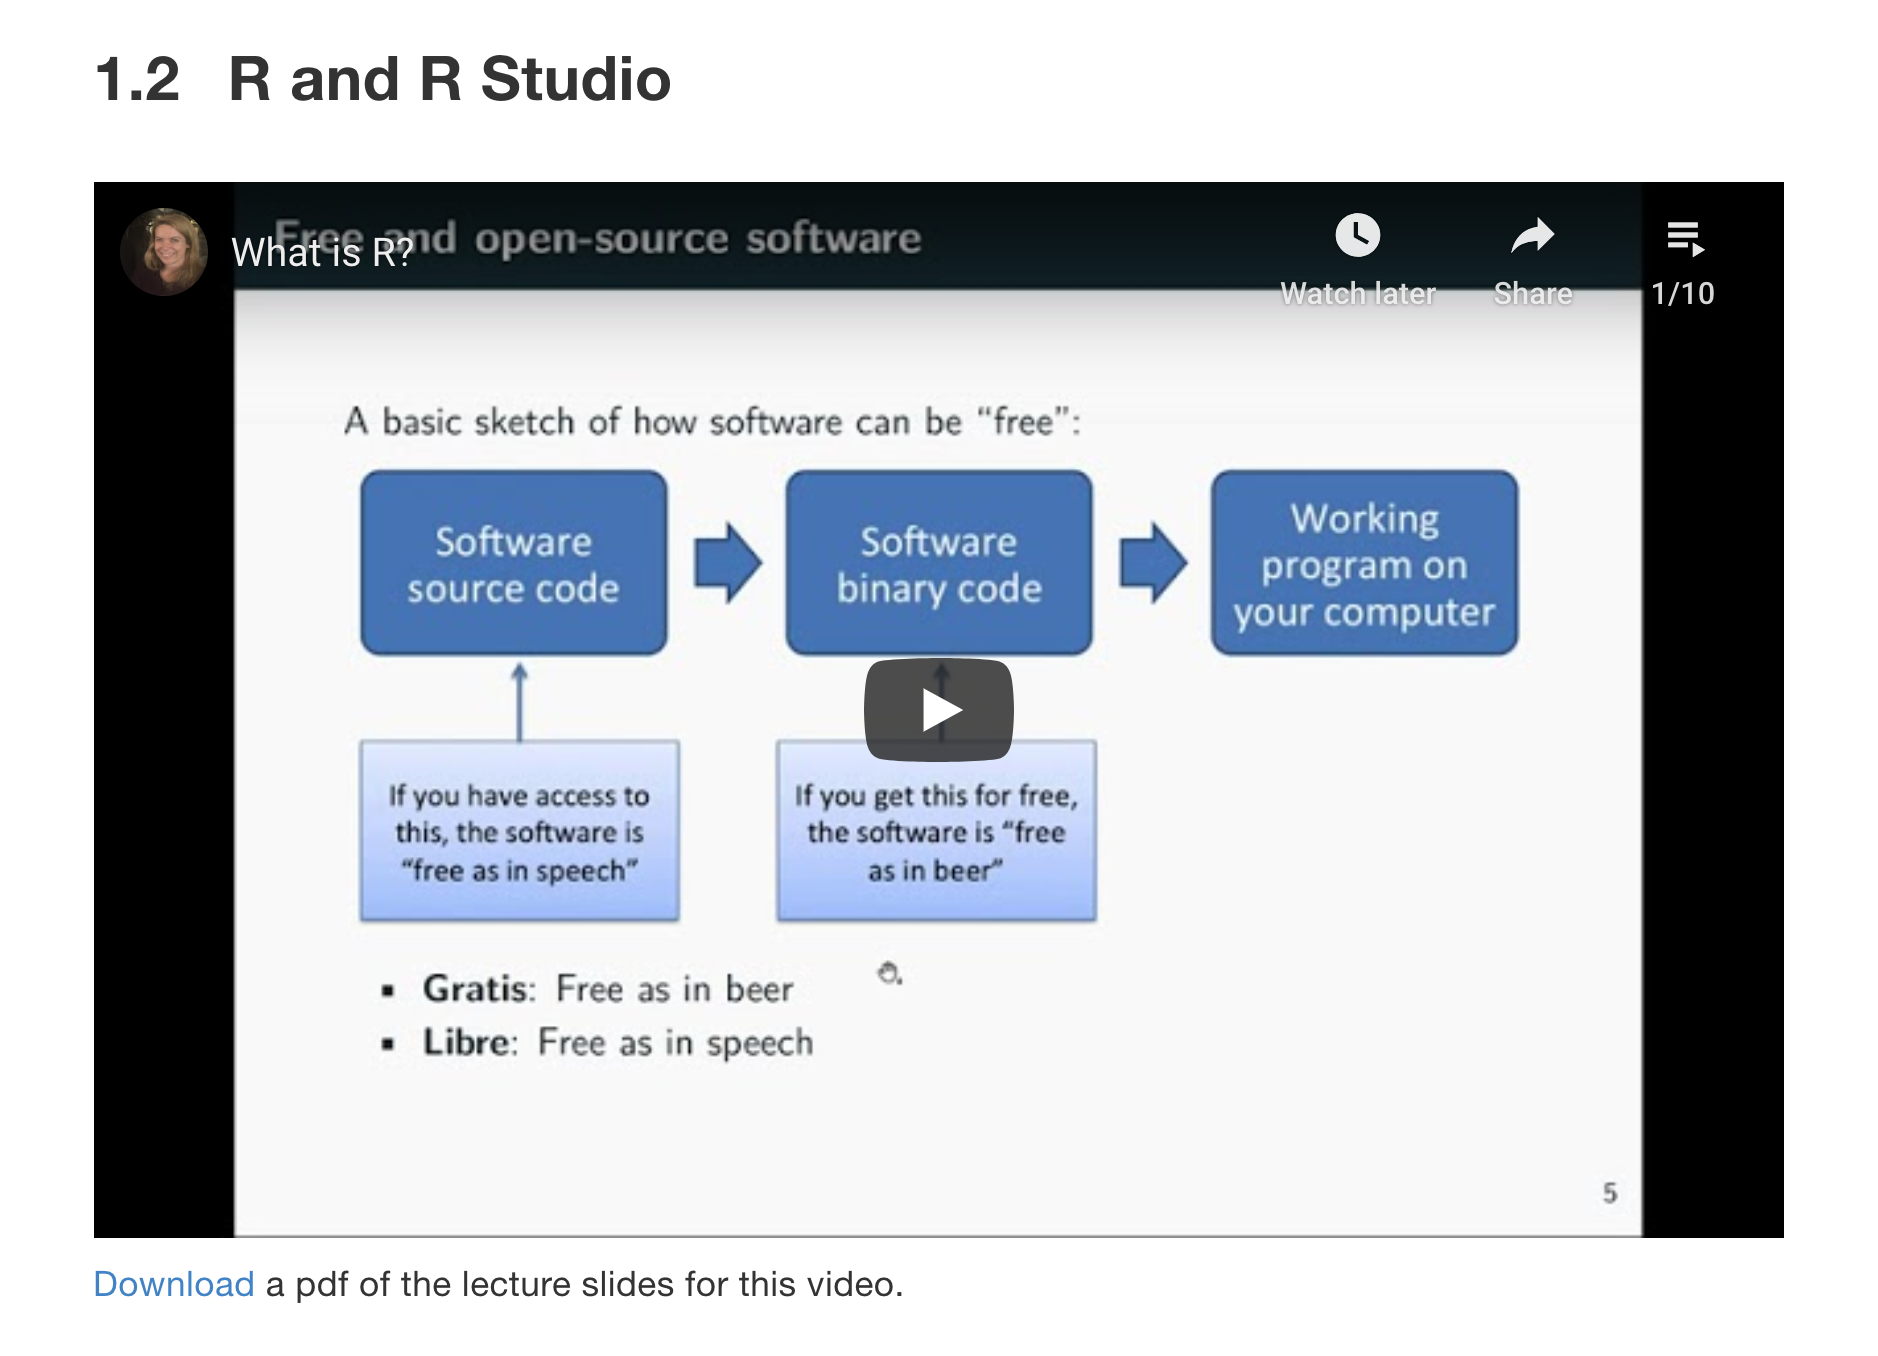
\includegraphics[width=300pt]{../figures/video_lecture} \end{center}

\end{frame}

\begin{frame}{Attendance and class participation}
\protect\hypertarget{attendance-and-class-participation-4}{}

\begin{center}
\includegraphics[width=300pt]{../figures/playlist_1} \end{center}

\end{frame}

\begin{frame}{Attendance and class participation}
\protect\hypertarget{attendance-and-class-participation-5}{}

\begin{center}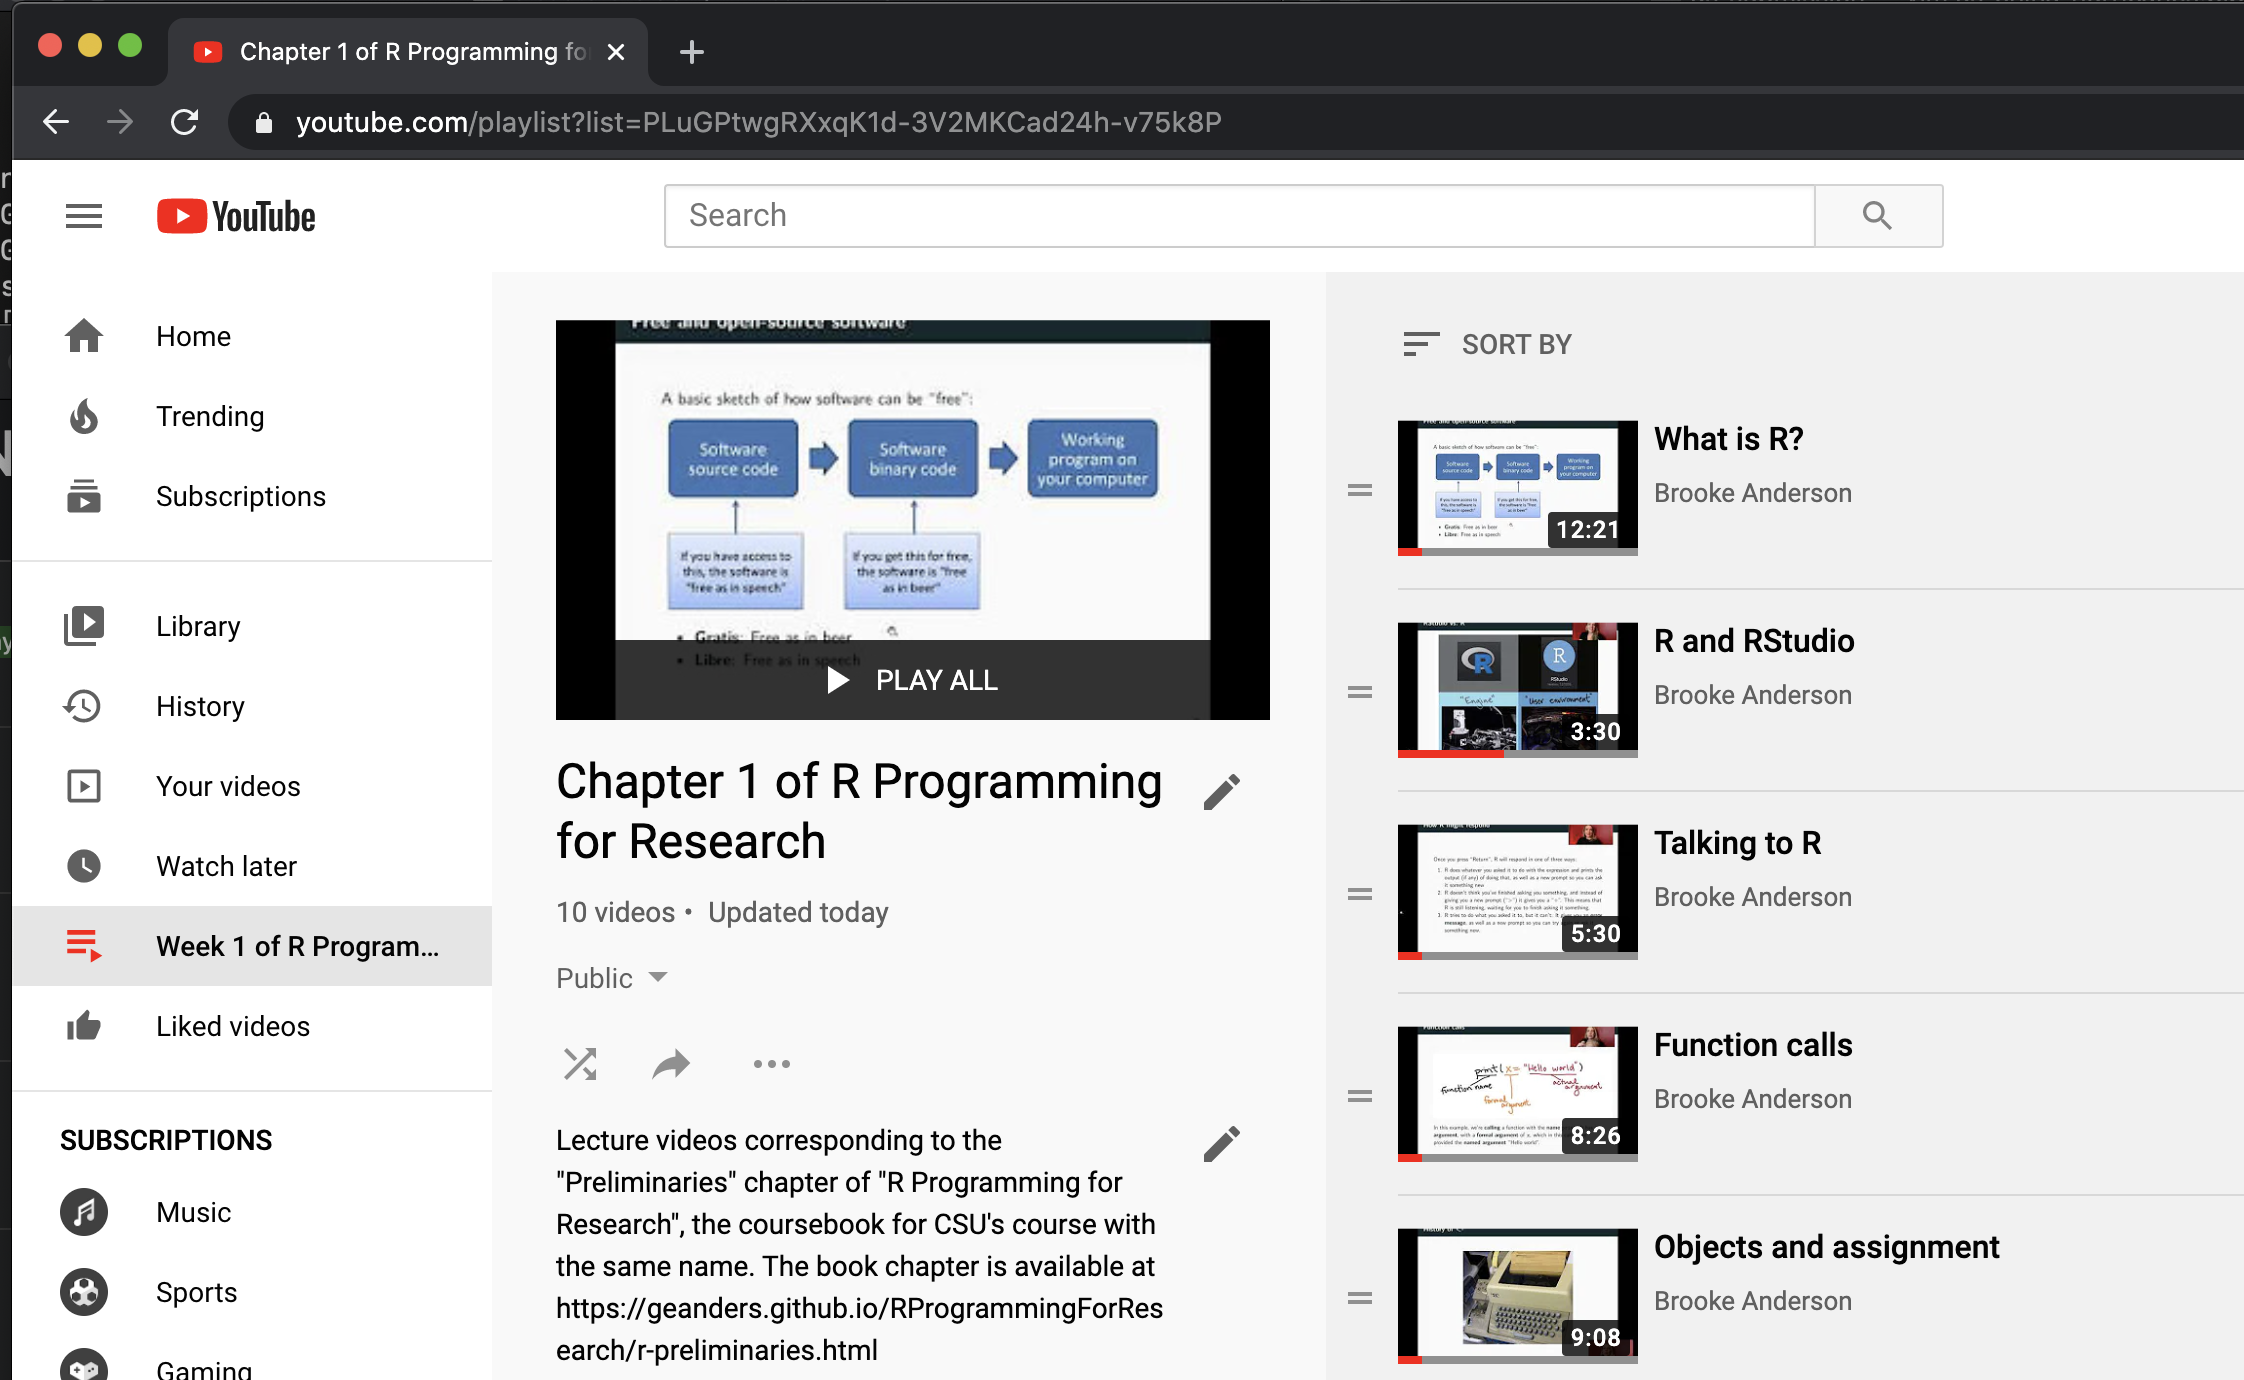
\includegraphics[width=300pt]{../figures/playlist_2} \end{center}

\end{frame}

\begin{frame}{Attendance and class participation}
\protect\hypertarget{attendance-and-class-participation-6}{}

You will be responsible for watching certain videos \emph{before} you
attend each live Zoom session. You will receive an email reminder with
the list of videos you need to watch before each meeting. There will be
about two hours worth of video lectures each week, broken into videos
about 10--15 minutes each.

This week, you will be responsible for watching the first nine videos in
Chapter 1 (``R Preliminaries'')

\end{frame}

\begin{frame}{Attendance and class participation---ERHS 535}
\protect\hypertarget{attendance-and-class-participationerhs-535}{}

If you are in \textbf{ERHS 535}, out of a possible 10 points for class
attendance, you will get:

\begin{itemize}
\tightlist
\item
  \textbf{10 points} if you miss two or fewer classes
\item
  \textbf{8 points} if you miss three classes
\item
  \textbf{6 points} if you miss four classes
\item
  \textbf{4 points} if you miss five classes
\item
  \textbf{2 points} if you miss six classes
\item
  \textbf{0 points} if you miss seven or more classes
\end{itemize}

\end{frame}

\begin{frame}{Attendance and class participation---ERHS 535}
\protect\hypertarget{attendance-and-class-participationerhs-535-1}{}

If you are in \textbf{ERHS 581A3}, out of a possible 10 points for class
attendance, you will get:

\begin{itemize}
\tightlist
\item
  \textbf{10 points} if you miss one or fewer classes
\item
  \textbf{8 points} if you miss two classes
\item
  \textbf{6 points} if you miss three classes
\item
  \textbf{4 points} if you miss four classes
\item
  \textbf{2 points} if you miss five classes
\item
  \textbf{0 points} if you miss six or more classes
\end{itemize}

\end{frame}

\begin{frame}{Attendance and class participation}
\protect\hypertarget{attendance-and-class-participation-7}{}

Excused absences:

\begin{itemize}
\tightlist
\item
  Attendance today (August 24) will not be counted
\item
  CSU-related: This is typically missing to attend a conference or for a
  field study for your research. To be excused, this requires a letter
  from your adviser.
\item
  Serious medical issue: To be excused, this requires a letter from a
  doctor or other medical professional.
\item
  For an absence to be excused, you must email me a copy of the letter
  by 5:00 pm the Friday afternoon following the class you missed.
\end{itemize}

\end{frame}

\begin{frame}{Weekly in-course group exercises}
\protect\hypertarget{weekly-in-course-group-exercises}{}

\begin{itemize}
\tightlist
\item
  As long as you attend the Zoom session and participate in these
  exercises, you will get full credit for this component.
\item
  \textbf{If you miss a Zoom meeting,} to get credit towards this
  component of your grade, you will need to turn in a few paragraphs
  describing what was covered in the exercise and what you learned.
\item
  To get credit for this, you must submit it to me by email by 5:00 pm
  the Friday afternoon after the class you missed.
\item
  All in-class exercises are included in the online course book at the
  end of the chapter on the associated material.
\end{itemize}

\end{frame}

\begin{frame}{Homework}
\protect\hypertarget{homework}{}

\begin{itemize}
\tightlist
\item
  In the first five weeks, there will be two homework assignments (see
  detailed schedule in the online course book).
\item
  These should be done individually.
\item
  Homeworks will be graded for correctness, but some partial credit will
  be given for questions you try but fail to answer correctly. Some of
  the exercises will not have ``correct'' answers, but instead will be
  graded on completeness.
\end{itemize}

\end{frame}

\begin{frame}{Homework}
\protect\hypertarget{homework-1}{}

\begin{center}\includegraphics[width=300pt]{../figures/find_homework} \end{center}

\end{frame}

\begin{frame}{Homework}
\protect\hypertarget{homework-2}{}

\begin{itemize}
\tightlist
\item
  Homework is due to me by email by 5:00 pm on Fridays (Friday,
  Sept.~11, and Friday, Sept.~25 are the due dates for the first five
  weeks of class).
\item
  Your grade will be reduced by 10 points for each day it is late, and
  will receive no credit if it is late by over a week.
\end{itemize}

\end{frame}

\begin{frame}{In-class quizzes}
\protect\hypertarget{in-class-quizzes}{}

\begin{itemize}
\tightlist
\item
  You will have quizzes weekly, starting next Wednesday (Sept.~2)
\item
  Quizzes will be on Wednesdays.

  \begin{itemize}
  \tightlist
  \item
    For students in the 10 AM cohort, the quizzes will be at the end of
    class (starting at 10:50 AM), and they will be allowed to continue
    working on the quiz until 11:10 AM.
  \item
    For students in the 11 AM cohort, the quizzes will be at the end of
    class (starting at 10:50 AM) you should plan to join Zoom early on
    Wednesdays (10:50 AM). Quizzes will start at this time, and you will
    have until 11:10 AM to finish the quiz.
  \end{itemize}
\item
  For students in ERHS 535, quizzes will continue until week 10 of the
  course
\end{itemize}

\end{frame}

\begin{frame}{In-class quizzes}
\protect\hypertarget{in-class-quizzes-1}{}

\begin{itemize}
\tightlist
\item
  Quizzes will be conducted through Google Forms. They will be
  immediately graded, and you will get back your grade and feedback as
  soon as you submit the quiz.
\item
  You must stay on Zoom while you complete the quiz.
\item
  A link to the quiz will be provided at 10:50 AM in the Zoom chat.
\end{itemize}

\end{frame}

\begin{frame}{In-class quizzes}
\protect\hypertarget{in-class-quizzes-2}{}

\begin{itemize}
\tightlist
\item
  Quiz questions will be multiple choice, matching, or similar styles of
  questions. The questions are designed so that each can be answered
  fairly quickly.
\item
  If you miss a class with a quiz, you may make it up during office
  hours on the week of the missed quiz. Except in exceptional
  circumstances, this will be the only time when make-up quizzes will be
  offered.
\end{itemize}

\end{frame}

\begin{frame}{In-class quizzes}
\protect\hypertarget{in-class-quizzes-3}{}

\begin{itemize}
\tightlist
\item
  There will be \emph{at least} 10 questions per quiz. Usually, there
  will be 12--15.
\item
  If you get, on average, 10 correct questions per quiz, you will get
  the maximum possible points for the quiz component of your grade.
\end{itemize}

\end{frame}

\begin{frame}{In-class quizzes}
\protect\hypertarget{in-class-quizzes-4}{}

For ERHS 535 (nine quizzes total):

\[
\mbox{Quiz grade} = 25 * \frac{\mbox{Number of correct quiz answers}}{90}
\]

For ERHS 581A3 (four quizzes total):

\[
\mbox{Quiz grade} = 40 * \frac{\mbox{Number of correct quiz answers}}{40}
\]

\textbf{Note:} You can not get more than the maximum of for this
component quiz component (25 points for ERHS 535 students, 40 points for
ERHS 581A3 students).

\end{frame}

\begin{frame}{In-class quizzes}
\protect\hypertarget{in-class-quizzes-5}{}

\begin{itemize}
\tightlist
\item
  The ``Vocabulary'' appendix of our online book has the list of
  material for which you will be responsible for this quiz.
\item
  Most of the functions and concepts will have been covered in class,
  but some may not.
\item
  You are responsible for going through the list and, if there are
  things you don't know or remember from class, learning them. To do
  this, you can use help functions in R, Google, StackOverflow, books on
  R, ask a friend, and any other resource you can find.
\end{itemize}

\end{frame}

\begin{frame}{In-class quizzes}
\protect\hypertarget{in-class-quizzes-6}{}

\begin{center}\includegraphics[width=300pt]{../figures/find_vocab} \end{center}

\end{frame}

\begin{frame}[fragile]{In-class quizzes}
\protect\hypertarget{in-class-quizzes-7}{}

An example of the vocabulary list:

\begin{itemize}
\tightlist
\item
  \texttt{mean()}
\item
  \texttt{read\_csv}, argument \texttt{skip\ =}
\item
  R object
\item
  open source software
\item
  Hadley Wickham
\end{itemize}

\end{frame}

\begin{frame}{In-class quizzes}
\protect\hypertarget{in-class-quizzes-8}{}

\begin{itemize}
\tightlist
\item
  Using R frequently in your research or other coursework will also help
  you prepare.
\item
  Working on your homework assignments will also help you prepare.
\end{itemize}

\end{frame}

\begin{frame}{What you have due soon}
\protect\hypertarget{what-you-have-due-soon}{}

\begin{itemize}
\tightlist
\item
  Wednesday, Sept.~4, during class: First in-class quiz. The
  ``Vocabulary'' appendix of our online book has the list of material
  for which you will be responsible for this quiz (Quiz 1 list).
\item
  Friday, Sept.~13: First homework is due by 5:00 pm by email.
\end{itemize}

\end{frame}

\end{document}
